\chapter{Introducción}\label{cap:intro}


En 1947, los físicos británicos G. Rochester y C. Butler, se hallaban tomando fotografías a una cámara de niebla, tratando de detectar partículas generadas por los rayos cósmicos al impactar sobre las moléculas de la atmósfera, cuando observaron un par de rastros inusuales. Esas marcas desconocidas sólo podían ser explicadas por el decaimiento de una partícula neutra con masa mil veces mayor que la del electrón. Decidieron repetir el experimento en el Observatorio \textit{Pic du Midi}, situado a 2900 metros de altura en los Pirineos franceses. De esta manera, al incrementar la altitud, el flujo del rayo cósmico aumenta, facilitando que las partículas lleguen al detector.

Gracias a ello, consiguieron reproducir el experimento detectando decenas de estas nuevas partículas. Concluyeron que la partícula en decaimiento se trataba de un nuevo tipo de mesón, al que posteriormente se denominó mesón K, de ahí que también se la conozca como kaón. Además, se predijo que los mesones existían fugazmente en el núcleo para explicar por qué los nucleones con carga similar se unían. El mesón K tenía propiedades inusuales, lo que supuso que los científicos de la época la bautizaran con el sobrenombre de ``extraña''.

En diciembre de ese mismo año, se hicieron públicas en la revista \textit{Nature} dos de las numerosas fotografías tomadas de la cámara de niebla, que se muestran a continuación:

\begin{figure}[h]
\centering
	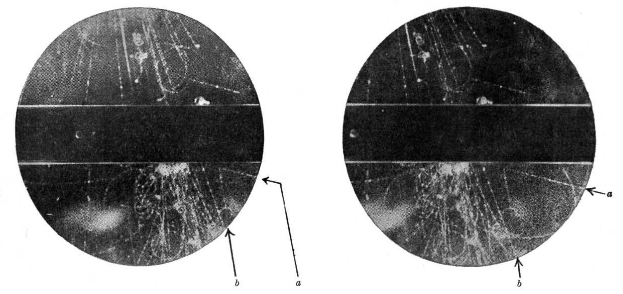
\includegraphics[width=0.6\textwidth]{{C:/Users/Carmen/Desktop/Universidad/TFG/Borradores/img/rochester1.PNG}}
	\caption[Primera fotografía estereoscópica] {Fotografía estereoscópica publicada en la revista Nature.
	\protect\footnotemark}
	\label{fig:rochester}
\end{figure}

\footnotetext{Imagen de la Revista Nature\cite{Nature1}}